\documentclass[english,12pt,a4paper,final]{article}
\usepackage[T1]{fontenc}
\usepackage[left=2cm, right=2cm, top=2cm, bottom=2cm]{geometry}
\usepackage{amssymb,graphicx,amsfonts,amsthm, tikz, listings}
\usepackage[bahasa]{babel}
\usetikzlibrary{shapes.geometric, arrows}
\begin{document}
	\begin{titlepage}
		\centering
		% TODO: \usepackage{graphicx} required
		
\includegraphics[width=0.15\textwidth]{logounesa.png}\par\vspace{1cm}
		{\Large \textsc{Laporan Tugas}\par}
		{\LARGE\bfseries Komputasi Matematika\par}
		{\large \textsc{4420102183}\par}
		\vspace{7cm}
		Oleh:\\[2ex]
		{\large\itshape Masukkan Nama Anda}\\
		23030214XXX\\
		MA - 2023X
		\vfill
		Dosen Pengampu:\par
		Dimas Avian \textsc{Maulana}, M.Si.\\
		% Dr. Rahmawati Erma Standsyah, M.Si.\\ (untuk 2023B)
	
		\vfill
		{\large\textsc{Universitas Negeri Surabaya} \par}
		{\large\textsc{Fakultas Matematika dan Ilmu Pengetahuan Alam} \par}
		{\large\textsc{Program Studi S1 Matematika} \par}
		\vspace{1cm}
		% Bottom of the page
		{\large \today\par}
	\end{titlepage}
\section{Permasalahan}
Uraikan masalah/tugas yang sedang Anda selesaikan disini
\section{\textit{Source Code}}
Tuliskan \textit{source code} disini. Berikut adalah contoh \textit{source code}:
\lstinputlisting[language=python]{epidemiology.py} %ganti epidemiology.py dengan file Anda

\section{Tangkapan Layar Hasil \textit{Running Source Code}}
\begin{figure}
	\centering
	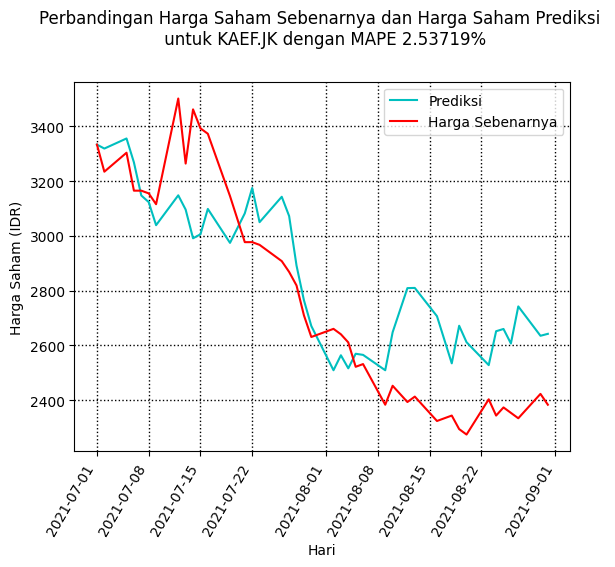
\includegraphics[width=\linewidth]{KAEF}
	\caption{Hasil running program dengan input xxx}
	\label{fig:kaef}
\end{figure}

\section{Penjelasan}
Berikan penjelasan terhadap program yang Anda kerjakan.

\begin{thebibliography}{9} 
	\bibitem{Azuela} Mariano Azuela, \textit{The Underdogs: A Novel of the Mexican Revolution}, trans. Beth Jorgensen (New York: The Modern Library, 2002). 
\end{thebibliography}
\end{document}